\subsection{Đặc tả chức năng (use-case)}
\subsubsection{Tính năng cho người dùng là khách hàng (customer)}
\begin{figure}[H]
    \centering
    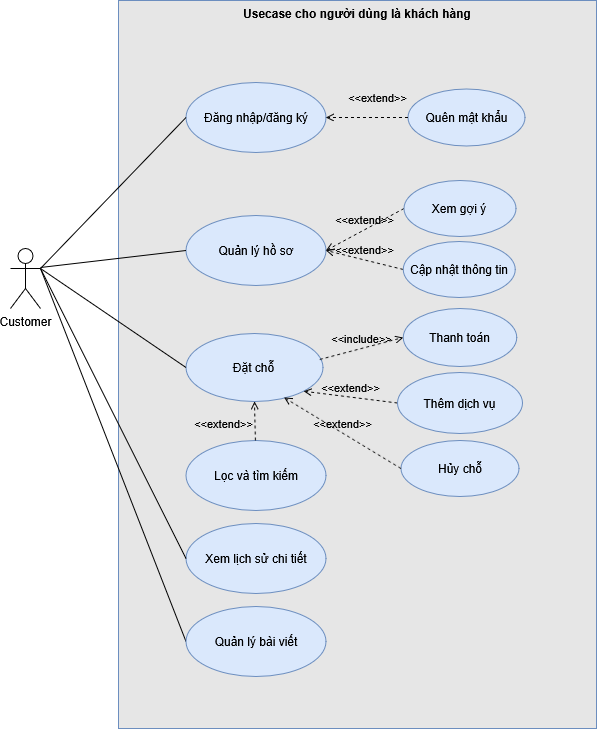
\includegraphics[width=0.8\textwidth]{Images/Chuong4/usecase-customer.png}
    \caption{Sơ đồ usecase cho người dùng là khách hàng}
    \label{fig:usecase-customer}
\end{figure}

\subsubsubsection{Use-case: Đăng nhập}

% \begin{figure}[H]
%     \centering
%     % Ghi chú: Hãy thay thế file ảnh này bằng sơ đồ use-case của chức năng Đăng nhập
%     \fbox{\parbox[c][5cm][c]{0.8\textwidth}{\centering Sơ đồ use-case: Đăng nhập}}
%     \caption{Use-case diagram của chức năng Đăng nhập}
%     \label{fig:login-uc}
% \end{figure}

\begin{table}[H]
\centering
\renewcommand{\arraystretch}{1.3}
\begin{tabular}{|p{4cm}|p{10cm}|}
\hline
\textbf{Tên Use-case} 
& Đăng nhập \\ 
\hline

\textbf{Mục tiêu} 
& Cho phép khách hàng đã có tài khoản truy cập vào hệ thống để sử dụng các chức năng cá nhân hóa. \\ 
\hline

\textbf{Tác nhân chính} 
& Khách hàng. \\ 
\hline

\textbf{Điều kiện tiên quyết} 
& Khách hàng đã đăng ký tài khoản thành công trên hệ thống. \\ 
\hline

\textbf{Điều kiện kết thúc} 
& 
\begin{itemize}
\item Khách hàng đăng nhập thành công và được chuyển hướng đến trang chính của hệ thống.
\item Khách hàng đăng nhập thất bại và nhận được thông báo lỗi.
\end{itemize} \\ 
\hline

\textbf{Luồng chính} 
& 
\begin{enumerate}
    \item Khách hàng truy cập trang đăng nhập.
    \item Khách hàng nhập thông tin.
    \item Khách hàng nhấn nút "Đăng nhập".
    \item Hệ thống xác thực thông tin đăng nhập .
    \item Hệ thống tạo một phiên làm việc (session/token) và chuyển hướng khách hàng đến trang chủ.
\end{enumerate} \\ 
\hline

\textbf{Luồng thay thế} 
& 
\begin{itemize}
    \item Thông tin không hợp lệ $\rightarrow$ Hệ thống hiển thị thông báo lỗi "Sai tên đăng nhập hoặc mật khẩu".
    \item Người dùng chọn \textit{Đăng nhập bằng Google} $\rightarrow$ Chuyển đến luồng xác thực của Google, sau khi thành công hệ thống tiến hành đăng nhập.
\end{itemize} \\ 
\hline

\textbf{Ràng buộc} 
& Mật khẩu phải được so sánh trên giá trị đã được mã hóa. Phiên làm việc có thời gian hết hạn. \\ 
\hline

\textbf{Ghi chú} 
& Không có. \\ 
\hline
\end{tabular}
\caption{Đặc tả chi tiết Use-case Đăng nhập}
\label{tab:login-spec}
\end{table}
\subsubsubsection{Use-case: Đăng ký tài khoản}

% \begin{figure}[H]
%     \centering
%     % Ghi chú: Hãy thay thế file ảnh này bằng sơ đồ use-case của chức năng Đăng ký
%     \fbox{\parbox[c][5cm][c]{0.8\textwidth}{\centering Sơ đồ use-case: Đăng ký tài khoản}}
%     \caption{Use-case diagram của chức năng Đăng ký tài khoản}
%     \label{fig:register-uc}
% \end{figure}

\begin{table}[H]
\centering
\renewcommand{\arraystretch}{1.3}
\begin{tabular}{|p{4cm}|p{10cm}|}
\hline
\textbf{Tên Use-case} 
& Đăng ký tài khoản \\ 
\hline

\textbf{Mục tiêu} 
& Cho phép người dùng mới tạo một tài khoản hợp lệ trên hệ thống để có thể sử dụng các chức năng \\ 
\hline

\textbf{Tác nhân chính} 
& Khách hàng (chưa có tài khoản). \\ 
\hline

\textbf{Điều kiện tiên quyết} 
& Người dùng chưa có tài khoản với email hoặc số điện thoại sắp đăng ký. \\ 
\hline

\textbf{Điều kiện kết thúc} 
& 
\begin{itemize}
\item Người dùng đăng ký thành công, tài khoản mới được tạo trong hệ thống và người dùng được đăng nhập.
\item Người dùng đăng ký thất bại do thông tin không hợp lệ hoặc đã tồn tại.
\end{itemize} \\ 
\hline

\textbf{Luồng chính} 
& 
\begin{enumerate}
    \item Người dùng truy cập trang đăng ký.
    \item Nhập các thông tin bắt buộc: Họ tên, email, mật khẩu.
    \item Nhấn nút "Đăng ký".
    \item Hệ thống kiểm tra tính hợp lệ và tính duy nhất của email.
    \item Hệ thống tạo tài khoản mới, mã hóa mật khẩu và lưu vào cơ sở dữ liệu.
    \item Hệ thống tự động đăng nhập và chuyển người dùng đến trang chủ.
\end{enumerate} \\ 
\hline

\textbf{Luồng thay thế} 
& 
\begin{itemize}
    \item Email đã tồn tại $\rightarrow$ Hệ thống hiển thị thông báo lỗi "Email này đã được sử dụng".
    \item Người dùng chọn \textit{Đăng ký bằng Google} $\rightarrow$ Chuyển đến luồng xác thực của Google, sau khi thành công hệ thống sẽ tạo tài khoản dựa trên thông tin Google trả về.
\end{itemize} \\ 
\hline

\textbf{Ràng buộc} 
& Mật khẩu phải được mã hóa an toàn. Email là duy nhất trên toàn hệ thống. \\ 
\hline

\textbf{Ghi chú} 
 \\ 
\hline
\end{tabular}
\caption{Đặc tả chi tiết Use-case Đăng ký tài khoản}
\label{tab:register-spec}
\end{table}
\subsubsubsection{Use-case: Tìm kiếm và Đặt chỗ}

% \begin{figure}[H]
%     \centering
%     % Ghi chú: Hãy thay thế file ảnh này bằng sơ đồ use-case của chức năng Tìm kiếm và Đặt chỗ
%     \fbox{\parbox[c][5cm][c]{0.8\textwidth}{\centering Sơ đồ use-case: Tìm kiếm và Đặt chỗ}}
%     \caption{Use-case diagram của chức năng Tìm kiếm và Đặt chỗ}
%     \label{fig:booking-uc}
% \end{figure}

\begin{table}[H]
\centering
\renewcommand{\arraystretch}{1.3}
\begin{tabular}{|p{4cm}|p{10cm}|}
\hline
\textbf{Tên Use-case} 
& Tìm kiếm và Đặt chỗ \\ 
\hline

\textbf{Mục tiêu} 
& Cho phép khách hàng tìm kiếm, lựa chọn, tùy chỉnh và đặt một không gian làm việc phù hợp với nhu cầu của mình. \\ 
\hline

\textbf{Tác nhân chính} 
& Khách hàng. \\ 
\hline

\textbf{Điều kiện tiên quyết} 
& Khách hàng đã đăng nhập vào hệ thống. \\ 
\hline

\textbf{Điều kiện kết thúc} 
& 
\begin{itemize}
\item Khách hàng đặt chỗ thành công, một booking mới được tạo với trạng thái "Chờ thanh toán".
\item Khách hàng thoát khỏi chức năng.
\end{itemize} \\ 
\hline

\textbf{Luồng chính} 
& 
\begin{enumerate}
    \item Khách hàng truy cập trang đặt chỗ.
    \item Khách hàng nhập các tiêu chí tìm kiếm: ngày, giờ, loại không gian,...
    \item Hệ thống hiển thị danh sách các không gian khả dụng.
    \item Khách hàng chọn một không gian để xem thông tin chi tiết.
    \item Hệ thống hiển thị trang xác nhận thông tin đặt chỗ. Tại đây, khách hàng có thể tùy chọn thêm các dịch vụ bổ sung (đồ uống, in ấn,...).
    \item Khách hàng nhấn "Xác nhận đặt chỗ".
    \item Hệ thống kiểm tra lại tính khả dụng để tránh xung đột.
    \item Hệ thống tạo một booking mới (bao gồm các dịch vụ bổ sung đã chọn) với trạng thái "Chờ thanh toán" và chuyển hướng khách hàng đến trang thanh toán.
\end{enumerate} \\ 
\hline

\textbf{Luồng thay thế} 
& 
 \\ 
\hline

\textbf{Ràng buộc} 
& Hệ thống phải sử dụng cơ chế khóa (locking) để đảm bảo không xảy ra tình trạng hai người cùng đặt một chỗ tại cùng một thời điểm (race condition). \\ 
\hline

\textbf{Ghi chú} 
& Chức năng "Thêm dịch vụ bổ sung" là một bước tùy chọn (extend) trong luồng đặt chỗ chính. \\ 
\hline
\end{tabular}
\caption{Đặc tả chi tiết Use-case Tìm kiếm và Đặt chỗ}
\label{tab:booking-spec}
\end{table}
\subsubsubsection{Use-case: Thanh toán đơn đặt chỗ}

% \begin{figure}[H]
%     \centering
%     % Ghi chú: Hãy thay thế file ảnh này bằng sơ đồ use-case của chức năng Thanh toán
%     \fbox{\parbox[c][5cm][c]{0.8\textwidth}{\centering Sơ đồ use-case: Thanh toán đơn đặt chỗ}}
%     \caption{Use-case diagram của chức năng Thanh toán đơn đặt chỗ}
%     \label{fig:payment-uc}
% \end{figure}

\begin{table}[H]
\centering
\renewcommand{\arraystretch}{1.3}
\begin{tabular}{|p{4cm}|p{10cm}|}
\hline
\textbf{Tên Use-case} 
& Thanh toán đơn đặt chỗ \\ 
\hline

\textbf{Mục tiêu} 
& Cho phép khách hàng hoàn tất việc thanh toán cho một đơn đặt chỗ đang ở trạng thái "Chờ thanh toán". \\ 
\hline

\textbf{Tác nhân chính} 
& Khách hàng. \\ 
\hline

\textbf{Điều kiện tiên quyết} 
& Khách hàng có một đơn đặt chỗ (booking) đang ở trạng thái "Chờ thanh toán". \\ 
\hline

\textbf{Điều kiện kết thúc} 
&
\begin{enumerate}
\item Khách hàng thanh toán thành công, trạng thái booking được cập nhật thành "Đã xác nhận".
\item Khách hàng thanh toán thất bại, booking vẫn ở trạng thái "Chờ thanh toán".
\item Khách hàng không thanh toán và booking hết hạn.
\end{enumerate}
\\ 
\hline

\textbf{Luồng chính} 
& 
\begin{enumerate}
    \item Khách hàng được chuyển đến trang thanh toán sau khi đặt chỗ, hoặc truy cập lại từ lịch sử đặt chỗ.
    \item Hệ thống hiển thị chi tiết đơn hàng và tổng số tiền cần thanh toán.
    \item Khách hàng hoàn tất thanh toán.
    \item Hệ thống nhận thông báo kết quả (webhook) từ MoMo.
    \item Hệ thống xác thực thông báo, cập nhật trạng thái booking thành "Đã xác nhận" và trạng thái thanh toán thành "Đã thanh toán".
    \item Hệ thống hiển thị trang thông báo thanh toán thành công cho khách hàng.
\end{enumerate} \\ 
\hline

\textbf{Luồng thay thế} 
& 
\begin{itemize}
    \item Thanh toán thất bại  $\rightarrow$ Hệ thống nhận thông báo thất bại, giữ nguyên trạng thái booking và hiển thị thông báo lỗi cho khách hàng.
\end{itemize} \\ 
\hline

\textbf{Ràng buộc} 
& Giao dịch thanh toán phải được xử lý một cách an toàn, có cơ chế xác thực webhook và chống xử lý trùng lặp (idempotency). \\ 
\hline

\textbf{Ghi chú} 
& Các booking ở trạng thái "Chờ thanh toán" sẽ tự động bị hủy sau một khoảng thời gian nhất định\\ 
\hline
\end{tabular}
\caption{Đặc tả chi tiết Use-case Thanh toán đơn đặt chỗ}
\label{tab:payment-spec}
\end{table}
\subsubsubsection{Use-case: Xem lịch sử đặt chỗ}

% \begin{figure}[H]
%     \centering
%     % Ghi chú: Hãy thay thế file ảnh này bằng sơ đồ use-case của chức năng Xem lịch sử
%     \fbox{\parbox[c][5cm][c]{0.8\textwidth}{\centering Sơ đồ use-case: Xem lịch sử đặt chỗ}}
%     \caption{Use-case diagram của chức năng Xem lịch sử đặt chỗ}
%     \label{fig:history-uc}
% \end{figure}

\begin{table}[H]
\centering
\renewcommand{\arraystretch}{1.3}
\begin{tabular}{|p{4cm}|p{10cm}|}
\hline
\textbf{Tên Use-case} 
& Xem lịch sử đặt chỗ \\ 
\hline

\textbf{Mục tiêu} 
& Cho phép khách hàng xem lại danh sách tất cả các đơn đặt chỗ đã thực hiện, bao gồm cả các giao dịch trong quá khứ và sắp tới. \\ 
\hline

\textbf{Tác nhân chính} 
& Khách hàng. \\ 
\hline

\textbf{Điều kiện tiên quyết} 
& Khách hàng đã đăng nhập vào hệ thống. \\ 
\hline

\textbf{Điều kiện kết thúc} 
& Khách hàng xem xong thông tin và thoát khỏi chức năng. \\ 
\hline

\textbf{Luồng chính} 
& 
\begin{enumerate}
    \item Khách hàng truy cập trang "Lịch sử đặt chỗ".
    \item Hệ thống truy vấn cơ sở dữ liệu và hiển thị danh sách các booking của khách hàng, được sắp xếp theo thời gian (mới nhất ở trên).
    \item Mỗi booking hiển thị các thông tin tóm tắt: mã đặt chỗ, tên không gian, thời gian, tổng tiền và trạng thái (Đã xác nhận, Đã hoàn thành, Đã hủy,...).
    \item Khách hàng có thể nhấn vào một booking để xem thông tin chi tiết.
\end{enumerate} \\ 
\hline

\textbf{Luồng thay thế} 
& 
\begin{itemize}
    \item Khách hàng chưa có booking nào $\rightarrow$ Hệ thống hiển thị thông báo "Bạn chưa có đơn đặt chỗ nào".
    \item Khách hàng sử dụng bộ lọc $\rightarrow$ Khách hàng có thể lọc danh sách booking theo trạng thái hoặc khoảng thời gian. Hệ thống hiển thị lại danh sách theo bộ lọc.
\end{itemize} \\ 
\hline

\textbf{Ràng buộc} 
\\ 
\hline

\textbf{Ghi chú} 
\\ 
\hline
\end{tabular}
\caption{Đặc tả chi tiết Use-case Xem lịch sử đặt chỗ}
\label{tab:history-spec}
\end{table}
\subsubsubsection{Use-case: Hủy đặt chỗ}

% \begin{figure}[H]
%     \centering
%     % Ghi chú: Hãy thay thế file ảnh này bằng sơ đồ use-case của chức năng Hủy đặt chỗ
%     \fbox{\parbox[c][5cm][c]{0.8\textwidth}{\centering Sơ đồ use-case: Hủy đặt chỗ}}
%     \caption{Use-case diagram của chức năng Hủy đặt chỗ}
%     \label{fig:cancel-uc}
% \end{figure}

\begin{table}[H]
\centering
\renewcommand{\arraystretch}{1.3}
\begin{tabular}{|p{4cm}|p{10cm}|}
\hline
\textbf{Tên Use-case} 
& Hủy đặt chỗ \\ 
\hline

\textbf{Mục tiêu} 
& Cho phép khách hàng gửi yêu cầu hủy một đơn đặt chỗ đã được xác nhận. \\ 
\hline

\textbf{Tác nhân chính} 
& Khách hàng. \\ 
\hline

\textbf{Điều kiện tiên quyết} 
& Khách hàng có một đơn đặt chỗ ở trạng thái "Đã xác nhận" và vẫn còn trong thời gian được phép hủy theo chính sách. \\ 
\hline

\textbf{Điều kiện kết thúc} 
&
\begin{enumerate}
\item Yêu cầu hủy được gửi thành công, booking chuyển sang trạng thái "Chờ xử lý hủy".
\item Khách hàng không thể hủy do không thỏa mãn điều kiện.
\end{enumerate}
\\ 
\hline

\textbf{Luồng chính} 
& 
\begin{enumerate}
    \item Khách hàng truy cập trang chi tiết của một đơn đặt chỗ.
    \item Khách hàng nhấn nút "Hủy đặt chỗ".
    \item Hệ thống kiểm tra các chính sách hủy hiện hành (ví dụ: hủy trước 24 giờ được hoàn 100\%).
    \item Hệ thống hiển thị một hộp thoại xác nhận, thông báo về chính sách sẽ được áp dụng (ví dụ: "Bạn sẽ được hoàn 80\% giá trị đơn hàng. Bạn có chắc chắn muốn hủy?").
    \item Khách hàng nhấn "Xác nhận hủy".
    \item Hệ thống cập nhật trạng thái booking thành "Đã hủy" và tạo một yêu cầu hoàn tiền (nếu có).
    \item Hệ thống hiển thị thông báo hủy thành công.
\end{enumerate} \\ 
\hline

\textbf{Luồng thay thế} 
& 
\begin{itemize}
    \item Booking không đủ điều kiện để hủy (ví dụ: đã quá sát giờ bắt đầu) $\rightarrow$ Nút "Hủy đặt chỗ" bị vô hiệu hóa hoặc hệ thống hiển thị thông báo "Đã quá thời gian cho phép hủy".
    \item Khách hàng nhấn "Không" trong hộp thoại xác nhận $\rightarrow$ Quy trình hủy kết thúc, booking không thay đổi trạng thái.
\end{itemize} \\ 
\hline

\textbf{Ràng buộc} 
& Các chính sách hủy phải được cấu hình rõ ràng trong hệ thống. \\ 
\hline

\textbf{Ghi chú} 
& - \\ 
\hline
\end{tabular}
\caption{Đặc tả chi tiết Use-case Hủy đặt chỗ}
\label{tab:cancel-spec}
\end{table}
\subsubsubsection{Use-case: Xem gợi ý kết nối}

% \begin{figure}[H]
%     \centering
%     % Ghi chú: Hãy thay thế file ảnh này bằng sơ đồ use-case của chức năng Gợi ý kết nối
%     \fbox{\parbox[c][5cm][c]{0.8\textwidth}{\centering Sơ đồ use-case: Xem gợi ý kết nối}}
%     \caption{Use-case diagram của chức năng Xem gợi ý kết nối}
%     \label{fig:matching-uc}
% \end{figure}

\begin{table}[H]
\centering
\renewcommand{\arraystretch}{1.3}
\begin{tabular}{|p{4cm}|p{10cm}|}
\hline
\textbf{Tên Use-case} 
& Xem gợi ý kết nối \\ 
\hline

\textbf{Mục tiêu} 
& Gợi ý cho khách hàng danh sách các thành viên khác có sự tương đồng về kỹ năng hoặc sở thích, nhằm thúc đẩy giao lưu và hợp tác. \\ 
\hline

\textbf{Tác nhân chính} 
& Khách hàng. \\ 
\hline

\textbf{Điều kiện tiên quyết} 
& Khách hàng đã đăng nhập và đã cập nhật thông tin kỹ năng/sở thích trong hồ sơ cá nhân. \\ 
\hline

\textbf{Điều kiện kết thúc} 
& Khách hàng xem xong danh sách gợi ý và có thể truy cập vào hồ sơ của người được gợi ý. \\ 
\hline

\textbf{Luồng chính} 
& 
\begin{enumerate}
    \item Khách hàng truy cập trang "Kết nối" hoặc "Gợi ý".
    \item Hệ thống lấy thông tin về kỹ năng và sở thích từ hồ sơ của khách hàng hiện tại.
    \item Hệ thống thực hiện thuật toán tính điểm tương đồng với các thành viên khác.
    \item Hệ thống hiển thị danh sách những thành viên có điểm tương đồng cao nhất.
    \item Mỗi thành viên trong danh sách hiển thị thông tin tóm tắt như tên, ảnh đại diện, và các kỹ năng/sở thích chung.
    \item Khách hàng có thể nhấn vào một thành viên để xem hồ sơ chi tiết (nếu người đó cho phép).
\end{enumerate} \\ 
\hline

\textbf{Luồng thay thế} 
& 
 \\ 
\hline

\textbf{Ràng buộc} 
\\ 
\hline

\textbf{Ghi chú} 
 \\ 
\hline
\end{tabular}
\caption{Đặc tả chi tiết Use-case Xem gợi ý kết nối}
\label{tab:matching-spec}
\end{table}
\subsubsection{Tính năng cho người dùng là nhân viên (staff)}
\begin{figure}[H]
    \centering
    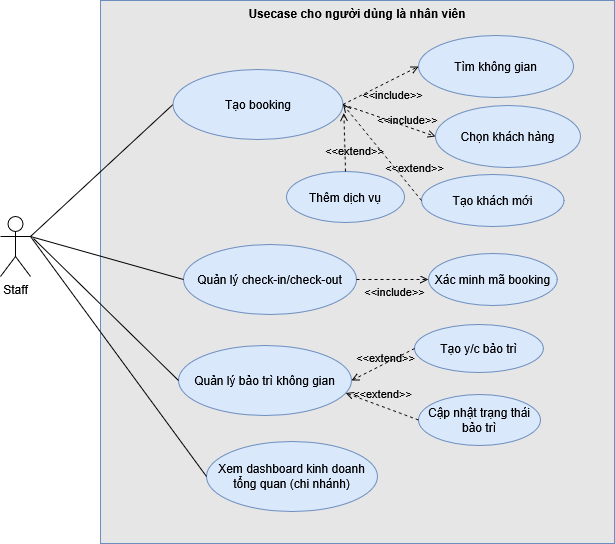
\includegraphics[width=0.8\textwidth]{Images/Chuong4/usecase-staff.png}
    \caption{Sơ đồ usecase cho người dùng là nhân viên}
    \label{fig:usecase-staff}
\end{figure}
\subsubsubsection{Use-case: Tạo booking cho khách}

% \begin{figure}[H]
%     \centering
%     % Ghi chú: Hãy thay thế fbox này bằng sơ đồ use-case của chức năng Tạo booking cho khách
%     \fbox{\parbox[c][5cm][c]{0.8\textwidth}{\centering Sơ đồ use-case: Tạo booking cho khách}}
%     \caption{Use-case diagram của chức năng Tạo booking cho khách}
%     \label{fig:staff-booking-uc}
% \end{figure}

\begin{table}[H]
\centering
\renewcommand{\arraystretch}{1.3}
\begin{tabular}{|p{4cm}|p{10cm}|}
\hline
\textbf{Tên Use-case} 
& Tạo booking cho khách \\ 
\hline

\textbf{Mục tiêu} 
& Cho phép nhân viên tạo một đơn đặt chỗ mới thay mặt cho khách hàng, thường áp dụng cho khách đặt trực tiếp tại quầy hoặc qua điện thoại. \\ 
\hline

\textbf{Tác nhân chính} 
& Nhân viên (Staff). \\ 
\hline

\textbf{Điều kiện tiên quyết} 
& Nhân viên đã đăng nhập vào hệ thống với tài khoản được cấp quyền. \\ 
\hline

\textbf{Điều kiện kết thúc} 
&
\begin{enumerate}
\item Nhân viên tạo booking thành công, một đơn đặt chỗ mới được tạo và liên kết với thông tin khách hàng.
\item Nhân viên hủy bỏ thao tác và không có booking nào được tạo.
\end{enumerate}
\\ 
\hline

\textbf{Luồng chính} 
& 
\begin{enumerate}
    \item Nhân viên truy cập chức năng "Tạo booking mới".
    \item Nhân viên tìm kiếm và chọn thông tin khách hàng (nếu khách đã có tài khoản) hoặc nhập thông tin khách mới.
    \item Nhân viên thực hiện tìm kiếm không gian theo yêu cầu của khách (tương tự luồng tìm kiếm của khách hàng).
    \item Nhân viên chọn không gian và các dịch vụ bổ sung (nếu có).
    \item Nhân viên xác nhận thông tin và tạo booking.
    \item Hệ thống tạo một booking mới với trạng thái "Chờ thanh toán" (nếu khách chưa thanh toán) hoặc "Đã xác nhận" (nếu khách thanh toán ngay).
    \item Hệ thống hiển thị thông tin mã đặt chỗ cho nhân viên để cung cấp cho khách.
\end{enumerate} \\ 
\hline

\textbf{Luồng thay thế} 
& 
\begin{itemize}
    \item Không tìm thấy không gian phù hợp $\rightarrow$ Nhân viên thông báo cho khách và có thể thay đổi tiêu chí tìm kiếm.
    \item Không gian không còn khả dụng tại thời điểm xác nhận $\rightarrow$ Hệ thống báo lỗi và nhân viên phải chọn lại không gian khác.
\end{itemize} \\ 
\hline

\textbf{Ràng buộc} 
& Nhân viên chỉ có thể tạo booking cho các không gian thuộc chi nhánh mà mình đang làm việc. \\ 
\hline

\textbf{Ghi chú} 
& Chức năng này về cơ bản là tổng hợp luồng tìm kiếm và đặt chỗ của khách hàng, nhưng được thực hiện bởi nhân viên. \\ 
\hline
\end{tabular}
\caption{Đặc tả chi tiết Use-case Tạo booking cho khách}
\label{tab:staff-booking-spec}
\end{table}

\subsubsubsection{Use-case: Check-in và Check-out cho khách}

% \begin{figure}[H]
%     \centering
%     % Ghi chú: Hãy thay thế fbox này bằng sơ đồ use-case của chức năng Check-in/Check-out
%     \fbox{\parbox[c][5cm][c]{0.8\textwidth}{\centering Sơ đồ use-case: Check-in và Check-out}}
%     \caption{Use-case diagram của chức năng Check-in và Check-out cho khách}
%     \label{fig:checkin-uc}
% \end{figure}

\begin{table}[H]
\centering
\renewcommand{\arraystretch}{1.3}
\begin{tabular}{|p{4cm}|p{10cm}|}
\hline
\textbf{Tên Use-case} 
& Check-in và Check-out cho khách \\ 
\hline

\textbf{Mục tiêu} 
& Ghi nhận thời gian khách hàng bắt đầu và kết thúc sử dụng không gian đã đặt, phục vụ cho mục đích quản lý vận hành. \\ 
\hline

\textbf{Tác nhân chính} 
& Nhân viên (Staff). \\ 
\hline

\textbf{Điều kiện tiên quyết} 
&
\begin{enumerate}
\item Nhân viên đã đăng nhập.
\item Khách hàng có một booking hợp lệ (đã xác nhận và đúng khung giờ). 
\end{enumerate} \\ 
\hline

\textbf{Điều kiện kết thúc} 
& 
\begin{itemize}
\item Khách hàng được check-in thành công, trạng thái booking cập nhật thành "Đang sử dụng".
\item Khách hàng được check-out thành công, trạng thái booking cập nhật thành "Đã hoàn thành".
\end{itemize} \\ 
\hline

\textbf{Luồng chính (Check-in)} 
& 
\begin{enumerate}
    \item Nhân viên truy cập chức năng "Check-in".
    \item Nhân viên nhập mã đặt chỗ (booking code) do khách hàng cung cấp.
    \item Hệ thống tìm kiếm và hiển thị thông tin booking tương ứng.
    \item Hệ thống kiểm tra tính hợp lệ của booking (đã xác nhận, đúng giờ, chưa check-in).
    \item Nhân viên nhấn nút "Check-in".
    \item Hệ thống ghi nhận thời gian check-in và cập nhật trạng thái booking thành "Đang sử dụng".
\end{enumerate} \\ 
\hline

\textbf{Luồng thay thế} 
& 
\begin{itemize}
    \item 4a. Mã booking không hợp lệ $\rightarrow$ Hệ thống báo lỗi "Mã đặt chỗ không hợp lệ hoặc không tìm thấy".
    \item 4b. Booking chưa đến giờ check-in $\rightarrow$ Hệ thống báo lỗi "Chưa đến giờ check-in".
    \item 4c. Booking đã được check-in trước đó $\rightarrow$ Hệ thống báo lỗi "Đơn đặt chỗ này đã được check-in".
\end{itemize} \\ 
\hline

\textbf{Luồng phụ (Check-out)}
&
\begin{enumerate}
    \item Nhân viên tìm lại booking đang ở trạng thái "Đang sử dụng".
    \item Nhân viên nhấn nút "Check-out".
    \item Hệ thống ghi nhận thời gian check-out và cập nhật trạng thái booking thành "Đã hoàn thành".
    \item Hệ thống có thể gửi thông báo cho khách hàng về việc không check-out đúng giờ (nếu có).
\end{enumerate} \\
\hline

\textbf{Ràng buộc} 
& Một booking chỉ có thể được check-in một lần. \\ 
\hline

\textbf{Ghi chú} 
& - \\ 
\hline
\end{tabular}
\caption{Đặc tả chi tiết Use-case Check-in và Check-out cho khách}
\label{tab:checkin-spec}
\end{table}
\subsubsubsection{Use-case: Quản lý bảo trì không gian}

% \begin{figure}[H]
%     \centering
%     % Ghi chú: Hãy thay thế fbox này bằng sơ đồ use-case của chức năng Quản lý bảo trì
%     \fbox{\parbox[c][5cm][c]{0.8\textwidth}{\centering Sơ đồ use-case: Quản lý bảo trì}}
%     \caption{Use-case diagram của chức năng Quản lý bảo trì không gian}
%     \label{fig:maintenance-uc}
% \end{figure}

\begin{table}[H]
\centering
\renewcommand{\arraystretch}{1.3}
\begin{tabular}{|p{4cm}|p{10cm}|}
\hline
\textbf{Tên Use-case} 
& Quản lý bảo trì không gian \\ 
\hline

\textbf{Mục tiêu} 
& Cho phép nhân viên tạo hoặc xóa các lịch bảo trì cho một không gian làm việc, khiến không gian đó tạm thời không khả dụng để đặt chỗ. \\ 
\hline

\textbf{Tác nhân chính} 
& Nhân viên (Staff). \\ 
\hline

\textbf{Điều kiện tiên quyết} 
& Nhân viên đã đăng nhập vào hệ thống. \\ 
\hline

\textbf{Điều kiện kết thúc} 
& 
\item Một lịch bảo trì mới được tạo thành công.
\item Một lịch bảo trì hiện có được xóa hoặc cập nhật.
\\ 
\hline

\textbf{Luồng chính} 
& 
\begin{enumerate}
    \item Nhân viên truy cập chức năng "Quản lý bảo trì".
    \item Nhân viên chọn không gian làm việc cần bảo trì.
    \item Nhân viên nhập thời gian bắt đầu, thời gian kết thúc và lý do bảo trì.
    \item Nhân viên nhấn nút "Tạo lịch bảo trì".
    \item Hệ thống kiểm tra xem có booking nào bị xung đột với lịch bảo trì mới không.
    \item Hệ thống lưu lịch bảo trì mới vào cơ sở dữ liệu.
    \item Không gian làm việc tương ứng sẽ không hiển thị trong kết quả tìm kiếm của khách hàng trong khung giờ bảo trì.
\end{enumerate} \\ 
\hline

\textbf{Luồng thay thế} 
& 
\begin{itemize}
    \item 5a. Có booking bị xung đột $\rightarrow$ Hệ thống hiển thị cảnh báo "Khung giờ này đã có khách đặt. Không thể tạo lịch bảo trì." và không cho phép tạo.
\end{itemize} \\ 
\hline

\textbf{Ràng buộc} 
& Không thể tạo lịch bảo trì trùng với thời gian đã có booking được xác nhận. \\ 
\hline

\textbf{Ghi chú} 
& Chức năng này rất quan trọng để đảm bảo chất lượng dịch vụ và quản lý tài sản. \\ 
\hline
\end{tabular}
\caption{Đặc tả chi tiết Use-case Quản lý bảo trì không gian}
\label{tab:maintenance-spec}
\end{table}
\subsubsubsection{Use-case: Xem Dashboard vận hành}

% \begin{figure}[H]
%     \centering
%     % Ghi chú: Hãy thay thế fbox này bằng sơ đồ use-case của chức năng Xem Dashboard
%     \fbox{\parbox[c][5cm][c]{0.8\textwidth}{\centering Sơ đồ use-case: Xem Dashboard}}
%     \caption{Use-case diagram của chức năng Xem Dashboard vận hành}
%     \label{fig:dashboard-uc}
% \end{figure}

\begin{table}[H]
\centering
\renewcommand{\arraystretch}{1.3}
\begin{tabular}{|p{4cm}|p{10cm}|}
\hline
\textbf{Tên Use-case} 
& Xem Dashboard vận hành \\ 
\hline

\textbf{Mục tiêu} 
& Cung cấp cho nhân viên một cái nhìn tổng quan về các hoạt động vận hành chính đang diễn ra trong ngày tại chi nhánh. \\ 
\hline

\textbf{Tác nhân chính} 
& Nhân viên (Staff). \\ 
\hline

\textbf{Điều kiện tiên quyết} 
& Nhân viên đã đăng nhập vào hệ thống. \\ 
\hline

\textbf{Điều kiện kết thúc} 
& Nhân viên xem xong thông tin và thoát khỏi chức năng. \\ 
\hline

\textbf{Luồng chính} 
& 
\begin{enumerate}
    \item Nhân viên truy cập trang Dashboard.
    \item Hệ thống tự động tải và hiển thị các thông tin vận hành của chi nhánh trong ngày hôm nay, bao gồm:
    \begin{itemize}
        \item Số lượng booking sắp tới.
        \item Danh sách các booking đang được sử dụng (đã check-in).
        \item Số lượng booking đang chờ thanh toán tiền mặt.
        \item Tình trạng tổng quan của các không gian (số chỗ trống, số chỗ đang dùng).
    \end{itemize}
    \item Dữ liệu trên dashboard có thể tự động làm mới sau một khoảng thời gian nhất định.
\end{enumerate} \\ 
\hline

\textbf{Luồng thay thế} 
 \\ 
\hline

\textbf{Ràng buộc} 
& Dữ liệu hiển thị trên dashboard chỉ thuộc về chi nhánh mà nhân viên đó đang làm việc. \\ 
\hline

\textbf{Ghi chú} 
& Đây là chức năng chỉ đọc (read-only), giúp nhân viên nắm bắt nhanh tình hình công việc. \\ 
\hline
\end{tabular}
\caption{Đặc tả chi tiết Use-case Xem Dashboard vận hành}
\label{tab:dashboard-spec}
\end{table}
\subsubsection{Tính năng cho người dùng là Quản trị chi nhánh (Admin Branch)}
\begin{figure}[H]
    \centering
    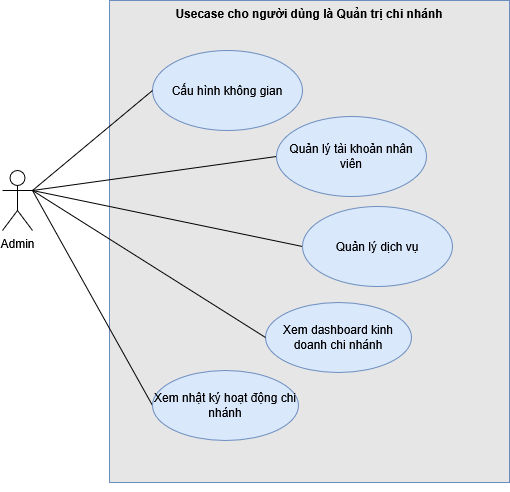
\includegraphics[width=0.8\textwidth]{Images/Chuong4/usecase-admin-branch.png}
    \caption{Sơ đồ usecase cho người dùng là quản lý chi nhánh}
    \label{fig:usecase-admin-branch}
\end{figure}
\subsubsubsection{Use-case: Quản lý giá và dịch vụ}

% \begin{figure}[H]
%     \centering
%     % Ghi chú: Hãy thay thế fbox này bằng sơ đồ use-case của chức năng Quản lý giá và dịch vụ
%     \fbox{\parbox[c][5cm][c]{0.8\textwidth}{\centering Sơ đồ use-case: Quản lý giá và dịch vụ}}
%     \caption{Use-case diagram của chức năng Quản lý giá và dịch vụ}
%     \label{fig:pricing-management-uc}
% \end{figure}

\begin{table}[H]
\centering
\renewcommand{\arraystretch}{1.3}
\begin{tabular}{|p{4cm}|p{10cm}|}
\hline
\textbf{Tên Use-case} 
& Quản lý giá và dịch vụ \\ 
\hline

\textbf{Mục tiêu} 
& Cho phép Quản lý chi nhánh thiết lập và cập nhật bảng giá cho thuê không gian cũng như giá của các dịch vụ bổ sung áp dụng riêng cho chi nhánh của mình. \\ 
\hline

\textbf{Tác nhân chính} 
& Quản lý chi nhánh (Branch Admin). \\ 
\hline

\textbf{Điều kiện tiên quyết} 
& Quản lý chi nhánh đã đăng nhập vào hệ thống với tài khoản có quyền quản trị chi nhánh. \\ 
\hline

\textbf{Điều kiện kết thúc} 
& 
\begin{itemize}
\item Bảng giá hoặc thông tin dịch vụ được cập nhật thành công.
\item Thao tác bị hủy bỏ và không có thay đổi nào được lưu.
\end{itemize} \\ 
\hline

\textbf{Luồng chính} 
& 
\begin{enumerate}
    \item Quản lý truy cập chức năng "Quản lý giá" hoặc "Quản lý dịch vụ".
    \item Hệ thống hiển thị danh sách các chính sách giá hoặc các dịch vụ hiện có của chi nhánh.
    \item Quản lý chọn "Thêm mới" hoặc "Chỉnh sửa" một mục cụ thể.
    \item Quản lý nhập các thông tin cần thiết (ví dụ: loại không gian, đơn vị thời gian, giá tiền; hoặc tên dịch vụ, đơn vị tính, giá tiền).
    \item Quản lý nhấn nút "Lưu".
    \item Hệ thống kiểm tra tính hợp lệ của dữ liệu và lưu các thay đổi vào cơ sở dữ liệu.
    \item Hệ thống hiển thị thông báo cập nhật thành công.
\end{enumerate} \\ 
\hline

\textbf{Luồng thay thế} 
& 
\begin{itemize}
    \item Dữ liệu không hợp lệ $\rightarrow$ Hệ thống hiển thị thông báo lỗi tại trường dữ liệu bị sai.
    \item Quản lý chọn "Xóa" một mục $\rightarrow$ Hệ thống yêu cầu xác nhận trước khi xóa vĩnh viễn.
\end{itemize} \\ 
\hline

\textbf{Ràng buộc} 
& Các thay đổi về giá sẽ được áp dụng cho các booking được tạo sau thời điểm cập nhật. \\ 
\hline

\textbf{Ghi chú} 
& Chức năng này cho phép mỗi chi nhánh có thể có chiến lược kinh doanh và giá cả linh hoạt. \\ 
\hline
\end{tabular}
\caption{Đặc tả chi tiết Use-case Quản lý giá và dịch vụ}
\label{tab:pricing-management-spec}
\end{table}
\subsubsubsection{Use-case: Xem báo cáo và lịch sử hoạt động}

% \begin{figure}[H]
%     \centering
%     % Ghi chú: Hãy thay thế fbox này bằng sơ đồ use-case của chức năng Xem báo cáo
%     \fbox{\parbox[c][5cm][c]{0.8\textwidth}{\centering Sơ đồ use-case: Xem báo cáo}}
%     \caption{Use-case diagram của chức năng Xem báo cáo và lịch sử hoạt động}
%     \label{fig:report-view-uc}
% \end{figure}

\begin{table}[H]
\centering
\renewcommand{\arraystretch}{1.3}
\begin{tabular}{|p{4cm}|p{10cm}|}
\hline
\textbf{Tên Use-case} 
& Xem báo cáo và lịch sử hoạt động \\ 
\hline

\textbf{Mục tiêu} 
& Cung cấp cho Quản lý chi nhánh cái nhìn tổng quan về hiệu quả hoạt động kinh doanh và khả năng tra cứu lại các hành động đã diễn ra trong chi nhánh. \\ 
\hline

\textbf{Tác nhân chính} 
& Quản lý chi nhánh (Branch Admin). \\ 
\hline

\textbf{Điều kiện tiên quyết} 
& Quản lý chi nhánh đã đăng nhập vào hệ thống. \\ 
\hline

\textbf{Điều kiện kết thúc} 
& Quản lý xem xong thông tin và thoát khỏi chức năng. \\ 
\hline

\textbf{Luồng chính} 
& 
\begin{enumerate}
    \item Quản lý truy cập mục "Báo cáo" hoặc "Lịch sử hoạt động".
    \item Quản lý chọn loại báo cáo muốn xem (ví dụ: Doanh thu, Tỷ lệ lấp đầy) và khoảng thời gian.
    \item Hệ thống truy vấn dữ liệu, tổng hợp và hiển thị kết quả dưới dạng biểu đồ và bảng số liệu.
    \item Đối với lịch sử hoạt động, hệ thống hiển thị danh sách các hành động (ai, làm gì, khi nào) đã được ghi lại.
    \item Quản lý có thể sử dụng các bộ lọc để tra cứu thông tin cụ thể.
\end{enumerate} \\ 
\hline

\textbf{Luồng thay thế} 
& 
\begin{itemize}
    \item 3a. Không có dữ liệu trong khoảng thời gian đã chọn $\rightarrow$ Hệ thống hiển thị thông báo "Không có dữ liệu để hiển thị".
\end{itemize} \\ 
\hline

\textbf{Ràng buộc} 
& Dữ liệu báo cáo và lịch sử hoạt động chỉ giới hạn trong phạm vi chi nhánh mà người quản lý đó phụ trách. \\ 
\hline

\textbf{Ghi chú} 
& Ở giai đoạn MVP, các báo cáo có thể ở mức độ tổng quan cơ bản. \\ 
\hline
\end{tabular}
\caption{Đặc tả chi tiết Use-case Xem báo cáo và lịch sử hoạt động}
\label{tab:report-view-spec}
\end{table}
\subsubsubsection{Use-case: Quản lý nhân viên chi nhánh}

% \begin{figure}[H]
%     \centering
%     % Ghi chú: Hãy thay thế fbox này bằng sơ đồ use-case của chức năng Quản lý nhân viên
%     \fbox{\parbox[c][5cm][c]{0.8\textwidth}{\centering Sơ đồ use-case: Quản lý nhân viên}}
%     \caption{Use-case diagram của chức năng Quản lý nhân viên chi nhánh}
%     \label{fig:staff-management-uc}
% \end{figure}

\begin{table}[H]
\centering
\renewcommand{\arraystretch}{1.3}
\begin{tabular}{|p{4cm}|p{10cm}|}
\hline
\textbf{Tên Use-case} 
& Quản lý nhân viên chi nhánh \\ 
\hline

\textbf{Mục tiêu} 
& Cho phép Quản lý chi nhánh tạo, cập nhật thông tin và quản lý trạng thái tài khoản của các nhân viên thuộc chi nhánh mình. \\ 
\hline

\textbf{Tác nhân chính} 
& Quản lý chi nhánh (Branch Admin). \\ 
\hline

\textbf{Điều kiện tiên quyết} 
& Quản lý chi nhánh đã đăng nhập vào hệ thống. \\ 
\hline

\textbf{Điều kiện kết thúc} 
& 
1. Thông tin của một nhân viên được tạo mới hoặc cập nhật thành công.
2. Trạng thái tài khoản của một nhân viên được thay đổi (ví dụ: khóa/mở khóa).
\\ 
\hline

\textbf{Luồng chính} 
& 
\begin{enumerate}
    \item Quản lý truy cập chức năng "Quản lý nhân viên".
    \item Hệ thống hiển thị danh sách các nhân viên hiện có trong chi nhánh.
    \item Quản lý chọn "Thêm nhân viên mới" hoặc chọn một nhân viên để "Chỉnh sửa".
    \item Quản lý điền các thông tin cần thiết (họ tên, email, mật khẩu ban đầu,...).
    \item Quản lý nhấn nút "Lưu".
    \item Hệ thống tạo mới hoặc cập nhật thông tin tài khoản nhân viên trong cơ sở dữ liệu.
    \item Hệ thống hiển thị thông báo thành công.
\end{enumerate} \\ 
\hline

\textbf{Luồng thay thế} 
& 
\begin{itemize}
    \item 3a. Quản lý chọn "Khóa tài khoản" $\rightarrow$ Hệ thống yêu cầu xác nhận, sau đó cập nhật trạng thái tài khoản thành "bị khóa", khiến nhân viên đó không thể đăng nhập.
    \item 6a. Email đã tồn tại $\rightarrow$ Hệ thống báo lỗi "Email đã được sử dụng cho một tài khoản khác".
\end{itemize} \\ 
\hline

\textbf{Ràng buộc} 
& Quản lý chi nhánh không thể xóa tài khoản nhân viên mà chỉ có thể khóa tài khoản để bảo toàn lịch sử dữ liệu. \\ 
\hline

\textbf{Ghi chú} 
& - \\ 
\hline
\end{tabular}
\caption{Đặc tả chi tiết Use-case Quản lý nhân viên chi nhánh}
\label{tab:staff-management-spec}
\end{table}
\subsubsubsection{Use-case: Quản lý không gian chi nhánh}

% \begin{figure}[H]
%     \centering
%     % Ghi chú: Hãy thay thế fbox này bằng sơ đồ use-case của chức năng Quản lý không gian
%     \fbox{\parbox[c][5cm][c]{0.8\textwidth}{\centering Sơ đồ use-case: Quản lý không gian}}
%     \caption{Use-case diagram của chức năng Quản lý không gian chi nhánh}
%     \label{fig:space-management-uc}
% \end{figure}

\begin{table}[H]
\centering
\renewcommand{\arraystretch}{1.3}
\begin{tabular}{|p{4cm}|p{10cm}|}
\hline
\textbf{Tên Use-case} 
& Quản lý không gian chi nhánh \\ 
\hline

\textbf{Mục tiêu} 
& Cho phép Quản lý chi nhánh cấu hình và cập nhật thông tin về các tầng và các không gian làm việc (chỗ ngồi, phòng họp) trong chi nhánh của mình. \\ 
\hline

\textbf{Tác nhân chính} 
& Quản lý chi nhánh (Branch Admin). \\ 
\hline

\textbf{Điều kiện tiên quyết} 
& Quản lý chi nhánh đã đăng nhập vào hệ thống. \\ 
\hline

\textbf{Điều kiện kết thúc} 
& 
1. Thông tin về một tầng hoặc không gian làm việc được tạo mới hoặc cập nhật thành công.
2. Một không gian làm việc được xóa khỏi hệ thống.
\\ 
\hline

\textbf{Luồng chính} 
& 
\begin{enumerate}
    \item Quản lý truy cập chức năng "Quản lý không gian".
    \item Hệ thống hiển thị cấu trúc các tầng và không gian làm việc của chi nhánh.
    \item Quản lý chọn "Thêm tầng mới", "Thêm không gian mới", hoặc chọn một mục để "Chỉnh sửa".
    \item Quản lý điền các thông tin chi tiết (ví dụ: số tầng, tải lên file sơ đồ SVG; hoặc mã không gian, loại, sức chứa, \texttt{svg\_element\_id}).
    \item Quản lý nhấn nút "Lưu".
    \item Hệ thống lưu thông tin vào cơ sở dữ liệu.
    \item Hệ thống hiển thị thông báo thành công và cập nhật lại giao diện.
\end{enumerate} \\ 
\hline

\textbf{Luồng thay thế} 
& 
\begin{itemize}
    \item 3a. Quản lý chọn "Xóa" một không gian $\rightarrow$ Hệ thống kiểm tra xem không gian đó có booking nào trong tương lai không. Nếu không, hệ thống yêu cầu xác nhận và tiến hành xóa. Nếu có, hệ thống từ chối xóa và hiển thị cảnh báo.
\end{itemize} \\ 
\hline

\textbf{Ràng buộc} 
& Việc tải lên file sơ đồ mặt bằng (SVG) và gán \texttt{svg\_element\_id} cho từng không gian là bắt buộc để tính năng bản đồ tương tác hoạt động. \\ 
\hline

\textbf{Ghi chú} 
& Đây là chức năng nền tảng, quyết định dữ liệu sẽ được hiển thị cho khách hàng như thế nào. \\ 
\hline
\end{tabular}
\caption{Đặc tả chi tiết Use-case Quản lý không gian chi nhánh}
\label{tab:space-management-spec}
\end{table}
\subsubsection{TÍnh năng cho người dùng là Quản trị Hệ thống (Admin System)}
\begin{figure}[H]
    \centering
    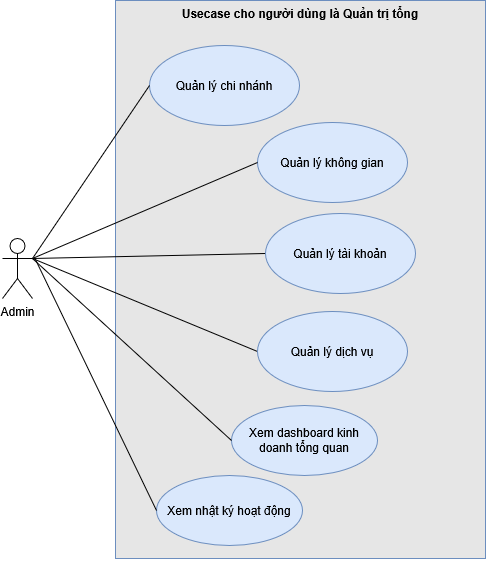
\includegraphics[width=0.8\textwidth]{Images/Chuong4/usecase-admin-system.png}
    \caption{Sơ đồ usecase cho người dùng là quản trị hệ thống}
    \label{fig:usecase-admin-system}
\end{figure}
\subsubsubsection{Use-case: Quản lý không gian (Toàn hệ thống)}



\begin{table}[H]
\centering
\renewcommand{\arraystretch}{1.3}
\begin{tabular}{|p{4cm}|p{10cm}|}
\hline
\textbf{Tên Use-case} 
& Quản lý không gian (Toàn hệ thống) \\ 
\hline

\textbf{Mục tiêu} 
& Cho phép Quản trị viên tạo, cập nhật và quản lý các đơn vị không gian ở cấp cao nhất, bao gồm các chi nhánh (branch) và các loại hình không gian (workspace type). \\ 
\hline

\textbf{Tác nhân chính} 
& Quản trị hệ thống (System Admin). \\ 
\hline

\textbf{Điều kiện tiên quyết} 
& Quản trị viên đã đăng nhập vào hệ thống. \\ 
\hline

\textbf{Điều kiện kết thúc} 
& 
\begin{itemize}
\item Một chi nhánh hoặc một loại hình không gian được tạo mới hoặc cập nhật thành công.
\item Thao tác bị hủy bỏ và không có thay đổi nào được lưu.
\end{itemize} \\ 
\hline

\textbf{Luồng chính} 
& 
\begin{enumerate}
    \item Quản trị viên truy cập chức năng "Quản lý không gian".
    \item Quản trị viên chọn mục "Quản lý chi nhánh" hoặc "Quản lý loại không gian".
    \item Hệ thống hiển thị danh sách các mục tương ứng hiện có.
    \item Quản trị viên chọn "Thêm mới" hoặc "Chỉnh sửa" một mục.
    \item Quản trị viên điền các thông tin cần thiết (ví dụ: tên chi nhánh, địa chỉ; hoặc tên loại không gian như "Chỗ ngồi cá nhân", "Phòng họp").
    \item Quản trị viên nhấn "Lưu".
    \item Hệ thống lưu thông tin vào cơ sở dữ liệu.
\end{enumerate} \\ 
\hline

\textbf{Luồng thay thế} 
& 
\begin{itemize}
    \item Quản trị viên chọn "Xóa" một mục $\rightarrow$ Hệ thống kiểm tra ràng buộc (không thể xóa chi nhánh nếu còn dữ liệu liên quan) và yêu cầu xác nhận trước khi xóa.
\end{itemize} \\ 
\hline

\textbf{Ràng buộc} 
& Việc tạo mới một chi nhánh là bước đầu tiên để Quản lý chi nhánh có thể cấu hình chi tiết hơn. \\ 
\hline

\textbf{Ghi chú} 
& Chức năng này khác với quản lý không gian của Branch Admin, vì nó tập trung vào các cấu trúc vĩ mô của toàn hệ thống. \\ 
\hline
\end{tabular}
\caption{Đặc tả chi tiết Use-case Quản lý không gian (Toàn hệ thống)}
\label{tab:sysadmin-space-spec}
\end{table}
\subsubsubsection{Use-case: Quản lý chính sách}



\begin{table}[H]
\centering
\renewcommand{\arraystretch}{1.3}
\begin{tabular}{|p{4cm}|p{10cm}|}
\hline
\textbf{Tên Use-case} 
& Quản lý chính sách \\ 
\hline

\textbf{Mục tiêu} 
& Cho phép Quản trị viên tạo và chỉnh sửa các chính sách áp dụng chung cho toàn hệ thống, chẳng hạn như chính sách hủy đặt chỗ và hoàn tiền. \\ 
\hline

\textbf{Tác nhân chính} 
& Quản trị hệ thống (System Admin). \\ 
\hline

\textbf{Điều kiện tiên quyết} 
& Quản trị viên đã đăng nhập vào hệ thống. \\ 
\hline

\textbf{Điều kiện kết thúc} 
& Một chính sách được tạo mới hoặc cập nhật thành công. \\ 
\hline

\textbf{Luồng chính} 
& 
\begin{enumerate}
    \item Quản trị viên truy cập chức năng "Quản lý chính sách".
    \item Hệ thống hiển thị danh sách các loại chính sách (ví dụ: Chính sách hủy).
    \item Quản trị viên chọn một chính sách để cấu hình.
    \item Quản trị viên định nghĩa các quy tắc (rule) cho chính sách. Ví dụ: đối với chính sách hủy, tạo quy tắc "Hủy trước 24 giờ, hoàn 100\%" hoặc "Hủy trong vòng 2 giờ sau khi đặt, hoàn 100\%".
    \item Quản trị viên lưu lại các quy tắc.
    \item Hệ thống cập nhật các quy tắc chính sách vào cơ sở dữ liệu.
\end{enumerate} \\ 
\hline

\textbf{Luồng thay thế} 
& 
\begin{itemize}
    \item 4a. Quản trị viên xóa một quy tắc $\rightarrow$ Hệ thống yêu cầu xác nhận và xóa quy tắc khỏi chính sách.
\end{itemize} \\ 
\hline

\textbf{Ràng buộc} 
& Các chính sách này sẽ được hệ thống tự động áp dụng khi khách hàng thực hiện các hành động tương ứng (ví dụ: hủy booking). \\ 
\hline

\textbf{Ghi chú} 
& - \\ 
\hline
\end{tabular}
\caption{Đặc tả chi tiết Use-case Quản lý chính sách}
\label{tab:policy-management-spec}
\end{table}
\subsubsubsection{Use-case: Quản lý dịch vụ}



\begin{table}[H]
\centering
\renewcommand{\arraystretch}{1.3}
\begin{tabular}{|p{4cm}|p{10cm}|}
\hline
\textbf{Tên Use-case} 
& Quản lý dịch vụ \\ 
\hline

\textbf{Mục tiêu} 
& Cho phép Quản trị viên định nghĩa các loại hình dịch vụ bổ sung mà các chi nhánh có thể cung cấp. \\ 
\hline

\textbf{Tác nhân chính} 
& Quản trị hệ thống (System Admin). \\ 
\hline

\textbf{Điều kiện tiên quyết} 
& Quản trị viên đã đăng nhập vào hệ thống. \\ 
\hline

\textbf{Điều kiện kết thúc} 
& Một loại hình dịch vụ được tạo mới, cập nhật hoặc xóa thành công. \\ 
\hline

\textbf{Luồng chính} 
& 
\begin{enumerate}
    \item Quản trị viên truy cập chức năng "Quản lý dịch vụ".
    \item Hệ thống hiển thị danh sách các loại hình dịch vụ hiện có (ví dụ: Đồ uống, In ấn, Gửi xe).
    \item Quản trị viên chọn "Thêm mới" hoặc "Chỉnh sửa" một loại hình.
    \item Quản trị viên nhập tên và mô tả cho loại hình dịch vụ.
    \item Quản trị viên nhấn "Lưu".
    \item Hệ thống lưu thông tin vào cơ sở dữ liệu.
\end{enumerate} \\ 
\hline

\textbf{Luồng thay thế} 
& 
\begin{itemize}
    \item 3a. Quản trị viên chọn "Xóa" $\rightarrow$ Hệ thống kiểm tra xem có dịch vụ nào đang sử dụng loại hình này không. Nếu không, hệ thống cho phép xóa.
\end{itemize} \\ 
\hline

\textbf{Ràng buộc} 
& Quản trị viên chỉ định nghĩa "loại hình" dịch vụ. Việc tạo các dịch vụ cụ thể và đặt giá cho chúng thuộc về Quản lý chi nhánh. \\ 
\hline

\textbf{Ghi chú} 
& Chức năng này giúp chuẩn hóa dữ liệu dịch vụ trên toàn hệ thống. \\ 
\hline
\end{tabular}
\caption{Đặc tả chi tiết Use-case Quản lý dịch vụ}
\label{tab:service-management-spec}
\end{table}
\subsubsubsection{Use-case: Quản lý người dùng (Toàn hệ thống)}


\begin{table}[H]
\centering
\renewcommand{\arraystretch}{1.3}
\begin{tabular}{|p{4cm}|p{10cm}|}
\hline
\textbf{Tên Use-case} 
& Quản lý người dùng (Toàn hệ thống) \\ 
\hline

\textbf{Mục tiêu} 
& Cho phép Quản trị viên quản lý tất cả các tài khoản người dùng trong hệ thống và gán vai trò (phân quyền) tương ứng cho họ. \\ 
\hline

\textbf{Tác nhân chính} 
& Quản trị hệ thống (System Admin). \\ 
\hline

\textbf{Điều kiện tiên quyết} 
& Quản trị viên đã đăng nhập vào hệ thống. \\ 
\hline

\textbf{Điều kiện kết thúc} 
& 
\begin{itemize}
\item Một tài khoản người dùng được tạo mới, cập nhật hoặc thay đổi trạng thái thành công.
\item Vai trò của một người dùng được thay đổi thành công.
\end{itemize} \\ 
\hline

\textbf{Luồng chính} 
& 
\begin{enumerate}
    \item Quản trị viên truy cập chức năng "Quản lý người dùng".
    \item Hệ thống hiển thị danh sách tất cả người dùng trên toàn hệ thống.
    \item Quản trị viên có thể tìm kiếm, lọc người dùng theo tên, email, vai trò hoặc chi nhánh.
    \item Quản trị viên chọn một người dùng để xem chi tiết.
    \item Từ trang chi tiết, quản trị viên có thể thực hiện các hành động: thay đổi vai trò, gán vào chi nhánh, khóa/mở khóa tài khoản.
    \item Quản trị viên lưu lại các thay đổi.
    \item Hệ thống cập nhật thông tin và quyền của người dùng tương ứng.
\end{enumerate} \\ 
\hline

\textbf{Luồng thay thế} 
& 
\begin{itemize}
    \item Gán vai trò không hợp lệ $\rightarrow$ Hệ thống báo lỗi.
\end{itemize} \\ 
\hline

\textbf{Ràng buộc} 
& Quản trị viên không thể xóa tài khoản của chính mình hoặc hạ quyền của tài khoản admin cuối cùng trong hệ thống. \\ 
\hline

\textbf{Ghi chú} 
& Đây là chức năng cốt lõi để duy trì cấu trúc phân quyền và bảo mật của toàn bộ hệ thống. \\ 
\hline
\end{tabular}
\caption{Đặc tả chi tiết Use-case Quản lý người dùng (Toàn hệ thống)}
\label{tab:sysadmin-user-spec}
\end{table}
\subsubsubsection{Use-case: Xem báo cáo doanh thu}


\begin{table}[H]
\centering
\renewcommand{\arraystretch}{1.3}
\begin{tabular}{|p{4cm}|p{10cm}|}
\hline
\textbf{Tên Use-case} 
& Xem báo cáo doanh thu \\ 
\hline

\textbf{Mục tiêu} 
& Cung cấp cho Quản trị viên cái nhìn tổng quan về tình hình tài chính của toàn bộ hệ thống. \\ 
\hline

\textbf{Tác nhân chính} 
& Quản trị hệ thống (System Admin). \\ 
\hline

\textbf{Điều kiện tiên quyết} 
& Quản trị viên đã đăng nhập vào hệ thống. \\ 
\hline

\textbf{Điều kiện kết thúc} 
& Quản trị viên xem xong thông tin và thoát khỏi chức năng. \\ 
\hline

\textbf{Luồng chính} 
& 
\begin{enumerate}
    \item Quản trị viên truy cập mục "Báo cáo doanh thu".
    \item Quản trị viên chọn khoảng thời gian và có thể lọc theo từng chi nhánh.
    \item Hệ thống truy vấn dữ liệu từ các giao dịch thanh toán đã hoàn tất.
    \item Hệ thống tổng hợp và hiển thị các số liệu: tổng doanh thu, doanh thu theo từng chi nhánh, doanh thu theo loại hình dịch vụ,...
    \item Dữ liệu được trình bày dưới dạng biểu đồ (đường, cột) và bảng số liệu chi tiết.
\end{enumerate} \\ 
\hline

\textbf{Luồng thay thế} 
& 
\begin{itemize}
    \item -
\end{itemize} \\ 
\hline

\textbf{Ràng buộc} 
& Dữ liệu báo cáo phải chính xác và được tổng hợp từ các nguồn dữ liệu đã được xác thực. \\ 
\hline

\textbf{Ghi chú} 
& Chức năng này hỗ trợ việc ra quyết định kinh doanh ở cấp cao. \\ 
\hline
\end{tabular}
\caption{Đặc tả chi tiết Use-case Xem báo cáo doanh thu}
\label{tab:revenue-report-spec}
\end{table}
\subsubsubsection{Use-case: Xem nhật ký hoạt động (Audit Log)}



\begin{table}[H]
\centering
\renewcommand{\arraystretch}{1.3}
\begin{tabular}{|p{4cm}|p{10cm}|}
\hline
\textbf{Tên Use-case} 
& Xem nhật ký hoạt động (Audit Log) \\ 
\hline

\textbf{Mục tiêu} 
& Cho phép Quản trị viên tra cứu và giám sát lại toàn bộ các hành động quan trọng đã diễn ra trên hệ thống, phục vụ cho việc truy vết sự cố và giám sát an ninh. \\ 
\hline

\textbf{Tác nhân chính} 
& Quản trị hệ thống (System Admin). \\ 
\hline

\textbf{Điều kiện tiên quyết} 
& Quản trị viên đã đăng nhập vào hệ thống. \\ 
\hline

\textbf{Điều kiện kết thúc} 
& Quản trị viên xem xong thông tin và thoát khỏi chức năng. \\ 
\hline

\textbf{Luồng chính} 
& 
\begin{enumerate}
    \item Quản trị viên truy cập chức năng "Nhật ký hoạt động".
    \item Hệ thống hiển thị danh sách các hành động đã được ghi lại, sắp xếp theo thời gian gần nhất.
    \item Mỗi bản ghi log bao gồm: người thực hiện, hành động (ví dụ: "tạo booking", "cập nhật giá"), đối tượng bị tác động, thời gian thực hiện, và địa chỉ IP (tùy chọn).
    \item Quản trị viên sử dụng các bộ lọc để tra cứu log theo người dùng, loại hành động, hoặc khoảng thời gian.
\end{enumerate} \\ 
\hline

\textbf{Luồng thay thế} 
& 
\begin{itemize}
    \item -
\end{itemize} \\ 
\hline

\textbf{Ràng buộc} 
& Dữ liệu Audit Log phải được lưu trữ một cách an toàn, không thể bị thay đổi hoặc xóa bởi bất kỳ vai trò nào, kể cả admin (trừ khi có cơ chế đặc biệt). \\ 
\hline

\textbf{Ghi chú} 
& Đây là một chức năng tối quan trọng cho việc quản trị và bảo mật hệ thống. \\ 
\hline
\end{tabular}
\caption{Đặc tả chi tiết Use-case Xem nhật ký hoạt động (Audit Log)}
\label{tab:audit-log-spec}
\end{table}